% ============================================================
% Question Bank: Modified ch03-08 Solving Real-World Problems with Rational Numbers
% Topic Title: Solving Real-World Problems with Rational Numbers — Alaska Contexts
% Culturally Responsive: Alaska (fishing, temperature, mushing, bush planes)
% Questions: 27 (15 MC + 6 SA + 6 Graphical)
% ============================================================

% --- Multiple Choice Questions (15) ---

\begin{practiceQuestion}{m-3-8-q01}{mc}
\begin{questionText}
A fisherman in Kodiak catches $48$ pounds of salmon and sells it for $\$5.75$ per pound. He also catches $32$ pounds of halibut and sells it for $\$8.25$ per pound. What is his total earnings?
\end{questionText}
\choiceA{$\$540.00$}
\choiceB{$\$264.00$}
\choiceC{$\$276.00$}
\choiceD{$\$504.00$}
\correctAnswer{A}
\explanation{Salmon: $48 \times 5.75 = \$276.00$. Halibut: $32 \times 8.25 = \$264.00$. Total: $276 + 264 = \$540.00$.}
\end{practiceQuestion}

\begin{practiceQuestion}{m-3-8-q02}{mc}
\begin{questionText}
The temperature in Fairbanks at $6{:}00$ a.m.\ was $-28°$F. By noon it had risen $15°$F. By midnight it dropped $22°$F from the noon reading. What was the midnight temperature?
\end{questionText}
\choiceA{$-13°$F}
\choiceB{$-35°$F}
\choiceC{$-9°$F}
\choiceD{$9°$F}
\correctAnswer{B}
\explanation{Noon: $-28 + 15 = -13°$F. Midnight: $-13 - 22 = -35°$F.}
\end{practiceQuestion}

\begin{practiceQuestion}{m-3-8-q03}{mc}
\begin{questionText}
A bush pilot flies $\dfrac{3}{4}$ of a $280$-mile route from Bethel to a remote village before stopping for fuel. How many miles remain?
\end{questionText}
\choiceA{$210$ miles}
\choiceB{$70$ miles}
\choiceC{$93\dfrac{1}{3}$ miles}
\choiceD{$140$ miles}
\correctAnswer{B}
\explanation{Distance flown: $\dfrac{3}{4} \times 280 = 210$ miles. Remaining: $280 - 210 = 70$ miles.}
\end{practiceQuestion}

\begin{practiceQuestion}{m-3-8-q04}{mc}
\begin{questionText}
During the Iditarod, a musher's dog team covers $62.5$ miles on Day $1$ and $48.75$ miles on Day $2$. If the total race is $975$ miles, how many miles remain after Day $2$?
\end{questionText}
\choiceA{$863.75$ miles}
\choiceB{$926.25$ miles}
\choiceC{$111.25$ miles}
\choiceD{$912.25$ miles}
\correctAnswer{A}
\explanation{Traveled: $62.5 + 48.75 = 111.25$ miles. Remaining: $975 - 111.25 = 863.75$ miles.}
\end{practiceQuestion}

\begin{practiceQuestion}{m-3-8-q05}{mc}
\begin{questionText}
A salmon cannery processes $4{,}250$ pounds of fish in $5$ equal batches. Each batch costs $\$1.20$ per pound to process. What is the cost per batch?
\end{questionText}
\choiceA{$\$5{,}100.00$}
\choiceB{$\$1{,}020.00$}
\choiceC{$\$850.00$}
\choiceD{$\$1{,}275.00$}
\correctAnswer{B}
\explanation{Pounds per batch: $4{,}250 \div 5 = 850$. Cost per batch: $850 \times 1.20 = \$1{,}020.00$.}
\end{practiceQuestion}

\begin{practiceQuestion}{m-3-8-q06}{mc}
\begin{questionText}
The depth of Denali base camp is at an elevation of $7{,}200$ feet. The summit of Denali is at $20{,}310$ feet. A climber at $14{,}800$ feet loses $2{,}350$ feet of elevation due to a storm retreat. What is the climber's new elevation?
\end{questionText}
\choiceA{$12{,}450$ feet}
\choiceB{$17{,}150$ feet}
\choiceC{$4{,}850$ feet}
\choiceD{$16{,}550$ feet}
\correctAnswer{A}
\explanation{$14{,}800 - 2{,}350 = 12{,}450$ feet.}
\end{practiceQuestion}

\begin{practiceQuestion}{m-3-8-q07}{mc}
\begin{questionText}
A fishing boat uses $12\dfrac{1}{2}$ gallons of fuel per hour. If the boat has $87\dfrac{1}{2}$ gallons of fuel, for how many hours can it operate?
\end{questionText}
\choiceA{$6$ hours}
\choiceB{$7$ hours}
\choiceC{$8$ hours}
\choiceD{$7\dfrac{1}{2}$ hours}
\correctAnswer{B}
\explanation{$87\dfrac{1}{2} \div 12\dfrac{1}{2} = \dfrac{175}{2} \div \dfrac{25}{2} = \dfrac{175}{2} \times \dfrac{2}{25} = 7$ hours.}
\end{practiceQuestion}

\begin{practiceQuestion}{m-3-8-q08}{mc}
\begin{questionText}
The average January temperature in Juneau is $28.4°$F. In Barrow, it is $-13.6°$F. How many degrees warmer is Juneau than Barrow?
\end{questionText}
\choiceA{$14.8°$F}
\choiceB{$42.0°$F}
\choiceC{$-42.0°$F}
\choiceD{$-14.8°$F}
\correctAnswer{B}
\explanation{$28.4 - (-13.6) = 28.4 + 13.6 = 42.0°$F.}
\end{practiceQuestion}

\begin{practiceQuestion}{m-3-8-q09}{mc}
\begin{questionText}
A bush plane carries cargo with a maximum payload of $1{,}200$ pounds. The pilot loads $3$ crates weighing $187\dfrac{1}{2}$ pounds each and $2$ barrels weighing $256\dfrac{1}{2}$ pounds each. How many more pounds can be loaded?
\end{questionText}
\choiceA{$124$ lb}
\choiceB{$125\dfrac{1}{2}$ lb}
\choiceC{$124\dfrac{1}{2}$ lb}
\choiceD{$126$ lb}
\correctAnswer{C}
\explanation{Crates: $3 \times 187\dfrac{1}{2} = 562\dfrac{1}{2}$ lb. Barrels: $2 \times 256\dfrac{1}{2} = 513$ lb. Total: $562\dfrac{1}{2} + 513 = 1{,}075\dfrac{1}{2}$ lb. Remaining: $1{,}200 - 1{,}075\dfrac{1}{2} = 124\dfrac{1}{2}$ lb.}
\end{practiceQuestion}

\begin{practiceQuestion}{m-3-8-q10}{mc}
\begin{questionText}
An Alaskan village records temperatures of $-18°$F, $-22°$F, $-15°$F, $-25°$F, and $-10°$F over $5$ days. What is the average temperature?
\end{questionText}
\choiceA{$-90°$F}
\choiceB{$-18°$F}
\choiceC{$18°$F}
\choiceD{$-20°$F}
\correctAnswer{B}
\explanation{Sum: $-18 + (-22) + (-15) + (-25) + (-10) = -90$. Average: $-90 \div 5 = -18°$F.}
\end{practiceQuestion}

\begin{practiceQuestion}{m-3-8-q11}{mc}
\begin{questionText}
A sled dog team is training. The team runs $\dfrac{2}{3}$ of a $45$-mile training loop, rests, then runs another $\dfrac{1}{5}$ of the total loop. How many miles has the team run in total?
\end{questionText}
\choiceA{$39$ miles}
\choiceB{$30$ miles}
\choiceC{$9$ miles}
\choiceD{$36$ miles}
\correctAnswer{A}
\explanation{First run: $\dfrac{2}{3} \times 45 = 30$ miles. Second run: $\dfrac{1}{5} \times 45 = 9$ miles. Total: $30 + 9 = 39$ miles.}
\end{practiceQuestion}

\begin{practiceQuestion}{m-3-8-q12}{mc}
\begin{questionText}
A fisherman earns $\$324.50$ on Monday, loses $\$78.25$ in equipment costs on Tuesday, earns $\$456.00$ on Wednesday, and pays $\$112.75$ for fuel on Thursday. What is his net earnings?
\end{questionText}
\choiceA{$\$589.50$}
\choiceB{$\$971.50$}
\choiceC{$\$691.50$}
\choiceD{$\$501.50$}
\correctAnswer{A}
\explanation{$324.50 - 78.25 + 456.00 - 112.75 = 589.50$.}
\end{practiceQuestion}

\begin{practiceQuestion}{m-3-8-q13}{mc}
\begin{questionText}
A bush plane descends at a rate of $350$ feet per minute from an altitude of $5{,}600$ feet. What is the altitude after $12$ minutes?
\end{questionText}
\choiceA{$1{,}400$ feet}
\choiceB{$4{,}200$ feet}
\choiceC{$9{,}800$ feet}
\choiceD{$1{,}200$ feet}
\correctAnswer{A}
\explanation{Descent: $350 \times 12 = 4{,}200$ feet. Altitude: $5{,}600 - 4{,}200 = 1{,}400$ feet.}
\end{practiceQuestion}

\begin{practiceQuestion}{m-3-8-q14}{mc}
\begin{questionText}
During a winter storm the temperature drops $3.5°$F every hour for $6$ hours. If it started at $8°$F, what is the final temperature?
\end{questionText}
\choiceA{$-13°$F}
\choiceB{$29°$F}
\choiceC{$-29°$F}
\choiceD{$-10°$F}
\correctAnswer{A}
\explanation{Drop: $3.5 \times 6 = 21°$F. Final: $8 - 21 = -13°$F.}
\end{practiceQuestion}

\begin{practiceQuestion}{m-3-8-q15}{mc}
\begin{questionText}
A fishing crew splits $\$2{,}856$ equally among $7$ members. Each member then pays $\$65$ for license fees. How much does each member keep?
\end{questionText}
\choiceA{$\$343$}
\choiceB{$\$408$}
\choiceC{$\$473$}
\choiceD{$\$278$}
\correctAnswer{A}
\explanation{Each share: $2{,}856 \div 7 = \$408$. After fees: $408 - 65 = \$343$.}
\end{practiceQuestion}

% --- Short Answer Questions (6) ---

\begin{practiceQuestion}{m-3-8-q16}{sa}
\begin{questionText}
A musher packs $15\dfrac{3}{4}$ pounds of dried fish, $8\dfrac{1}{2}$ pounds of dog kibble, and $6\dfrac{1}{4}$ pounds of supplies on a sled. What is the total weight of the packs?
\end{questionText}
\correctAnswer{$30\dfrac{1}{2}$ pounds}
\explanation{$15\dfrac{3}{4} + 8\dfrac{1}{2} + 6\dfrac{1}{4} = 15\dfrac{3}{4} + 8\dfrac{2}{4} + 6\dfrac{1}{4} = 29\dfrac{6}{4} = 30\dfrac{2}{4} = 30\dfrac{1}{2}$ pounds.}
\end{practiceQuestion}

\begin{practiceQuestion}{m-3-8-q17}{sa}
\begin{questionText}
A salmon hatchery releases $12{,}500$ fish on Monday and $9{,}750$ fish on Tuesday. If $\dfrac{2}{5}$ of the total released are expected to survive, how many fish are expected to survive?
\end{questionText}
\correctAnswer{$8{,}900$ fish}
\explanation{Total: $12{,}500 + 9{,}750 = 22{,}250$. Survivors: $\dfrac{2}{5} \times 22{,}250 = 8{,}900$.}
\end{practiceQuestion}

\begin{practiceQuestion}{m-3-8-q18}{sa}
\begin{questionText}
The high temperature in Anchorage was $12.4°$F. The overnight low was $-7.8°$F. What was the temperature change from high to low?
\end{questionText}
\correctAnswer{$-20.2°$F (a drop of $20.2°$F)}
\explanation{Change: $-7.8 - 12.4 = -20.2°$F.}
\end{practiceQuestion}

\begin{practiceQuestion}{m-3-8-q19}{sa}
\begin{questionText}
A bush pilot charges $\$3.45$ per mile for charter flights. A round trip from a village to Fairbanks is $184$ miles each way. What is the total cost of the round trip?
\end{questionText}
\correctAnswer{$\$1{,}269.60$}
\explanation{Round trip: $184 \times 2 = 368$ miles. Cost: $368 \times 3.45 = \$1{,}269.60$.}
\end{practiceQuestion}

\begin{practiceQuestion}{m-3-8-q20}{sa}
\begin{questionText}
A diver in the Bering Sea descends $\dfrac{5}{6}$ of a meter per second for $18$ seconds, then ascends $\dfrac{1}{3}$ of a meter per second for $12$ seconds. What is the diver's depth?
\end{questionText}
\correctAnswer{$-11$ meters (or $11$ meters below surface)}
\explanation{Descent: $\dfrac{5}{6} \times 18 = 15$ meters down $= -15$. Ascent: $\dfrac{1}{3} \times 12 = 4$ meters up. Net: $-15 + 4 = -11$ meters.}
\end{practiceQuestion}

\begin{practiceQuestion}{m-3-8-q21}{sa}
\begin{questionText}
An ice fishing tournament awards $\$12.50$ per pound for the heaviest fish. First place catches a fish weighing $28.4$ pounds. The entry fee is $\$75$. How much profit does first place earn?
\end{questionText}
\correctAnswer{$\$280.00$}
\explanation{Prize: $28.4 \times 12.50 = \$355.00$. Profit: $355 - 75 = \$280.00$.}
\end{practiceQuestion}

% --- Graphical Questions (3 GMC + 3 GSA) ---

\begin{practiceQuestion}{m-3-8-q22}{gmc}
\begin{questionText}
The bar graph shows the daily catch (in pounds) of a fishing crew over $4$ days. What is the average daily catch?

\begin{center}
\begin{tikzpicture}[scale=0.6]
  \draw[thick,->] (0,0) -- (0,6) node[above,font=\small] {Pounds};
  \draw[thick,->] (0,0) -- (6,0);
  \foreach \y in {1,...,5} \draw (-0.15,\y) -- (0.15,\y) node[left=4pt,font=\small] {$\pgfmathparse{int(\y*100)}\pgfmathresult$};
  \fill[funBlue] (0.5,0) rectangle (1.5,3.5);
  \fill[funRed] (2,0) rectangle (3,4.2);
  \fill[funGreen] (3.5,0) rectangle (4.5,2.8);
  \fill[funOrange] (5,0) rectangle (6,4.5);
  \node[below,font=\small] at (1,0) {Mon};
  \node[below,font=\small] at (2.5,0) {Tue};
  \node[below,font=\small] at (4,0) {Wed};
  \node[below,font=\small] at (5.5,0) {Thu};
\end{tikzpicture}
\end{center}
\end{questionText}
\choiceA{$375$ lb}
\choiceB{$350$ lb}
\choiceC{$400$ lb}
\choiceD{$325$ lb}
\correctAnswer{A}
\explanation{Mon: $350$, Tue: $420$, Wed: $280$, Thu: $450$ lb. Total: $1{,}500$. Average: $1{,}500 \div 4 = 375$ lb.}
\end{practiceQuestion}

\begin{practiceQuestion}{m-3-8-q23}{gmc}
\begin{questionText}
The line graph shows the temperature in Nome over $6$ hours. What was the total temperature change from Hour $0$ to Hour $6$?

\begin{center}
\begin{tikzpicture}[scale=0.7]
  \draw[thick,->] (0,-3.5) -- (0,2) node[above,font=\small] {°F};
  \draw[thick,->] (0,0) -- (7,0) node[right,font=\small] {Hours};
  \foreach \y in {-3,...,1} \draw (-0.15,\y) -- (0.15,\y) node[left=4pt,font=\small] {$\pgfmathparse{int(\y*5)}\pgfmathresult$};
  \foreach \x in {0,...,6} \draw (\x,-0.15) -- (\x,0.15) node[above=2pt,font=\small] {$\x$};
  \draw[thick,funBlue] (0,0.4) -- (1,0.8) -- (2,0) -- (3,-1.2) -- (4,-2.0) -- (5,-2.4) -- (6,-3);
  \foreach \x/\y in {0/0.4,1/0.8,2/0,3/-1.2,4/-2.0,5/-2.4,6/-3} \fill[funBlue] (\x,\y) circle (0.08);
\end{tikzpicture}
\end{center}
\end{questionText}
\choiceA{$-17°$F}
\choiceB{$17°$F}
\choiceC{$-15°$F}
\choiceD{$-13°$F}
\correctAnswer{A}
\explanation{Hour $0$: $2°$F. Hour $6$: $-15°$F. Change: $-15 - 2 = -17°$F.}
\end{practiceQuestion}

\begin{practiceQuestion}{m-3-8-q24}{gmc}
\begin{questionText}
The table shows fuel costs for bush plane routes. Which route has the lowest cost per mile?

\begin{center}
\begin{tabular}{|l|c|c|}
\hline
\textbf{Route} & \textbf{Distance (mi)} & \textbf{Fuel Cost} \\
\hline
Bethel–Aniak & $120$ & $\$336.00$ \\ \hline
Kodiak–Homer & $95$ & $\$285.00$ \\ \hline
Juneau–Sitka & $85$ & $\$229.50$ \\ \hline
\end{tabular}
\end{center}
\end{questionText}
\choiceA{Bethel–Aniak}
\choiceB{Kodiak–Homer}
\choiceC{Juneau–Sitka}
\choiceD{They are all equal}
\correctAnswer{C}
\explanation{Bethel–Aniak: $336 \div 120 = \$2.80$/mi. Kodiak–Homer: $285 \div 95 = \$3.00$/mi. Juneau–Sitka: $229.50 \div 85 = \$2.70$/mi. Juneau–Sitka has the lowest cost per mile.}
\end{practiceQuestion}

\begin{practiceQuestion}{m-3-8-q25}{gsa}
\begin{questionText}
The table shows the weight of salmon caught each day of a $5$-day fishing trip. Find the total weight and the average weight per day.

\begin{center}
\begin{tabular}{|l|c|}
\hline
\textbf{Day} & \textbf{Weight (lb)} \\
\hline
Day 1 & $34.5$ \\ \hline
Day 2 & $28.75$ \\ \hline
Day 3 & $41.25$ \\ \hline
Day 4 & $36.0$ \\ \hline
Day 5 & $29.5$ \\ \hline
\end{tabular}
\end{center}
\end{questionText}
\correctAnswer{Total: $170$ lb; Average: $34$ lb per day}
\explanation{$34.5 + 28.75 + 41.25 + 36.0 + 29.5 = 170$ lb. Average: $170 \div 5 = 34$ lb.}
\end{practiceQuestion}

\begin{practiceQuestion}{m-3-8-q26}{gsa}
\begin{questionText}
The diagram shows a bush plane's altitude changes. What is the plane's final altitude?

\begin{center}
\begin{tikzpicture}[scale=0.5]
  \draw[thick,->] (0,0) -- (12,0) node[right,font=\small] {Time};
  \draw[thick,->] (0,0) -- (0,7) node[above,font=\small] {Altitude (ft)};
  \foreach \y in {1,...,6} \draw (-0.2,\y) -- (0.2,\y) node[left=4pt,font=\small] {$\pgfmathparse{int(\y*1000)}\pgfmathresult$};
  \draw[very thick,funBlue] (0,0) -- (3,5) node[above,font=\small] {Climb} -- (6,5) node[above,font=\small] {Cruise} -- (9,2) node[above right,font=\small] {Descend} -- (11,2) node[above,font=\small] {Level};
  \fill[funBlue] (0,0) circle (0.12);
  \fill[funBlue] (11,2) circle (0.12);
\end{tikzpicture}
\end{center}
\end{questionText}
\correctAnswer{$2{,}000$ feet}
\explanation{The plane climbs to $5{,}000$ feet, cruises, descends to $2{,}000$ feet, and levels off at $2{,}000$ feet.}
\end{practiceQuestion}

\begin{practiceQuestion}{m-3-8-q27}{gsa}
\begin{questionText}
The number line models a musher's daily progress and setbacks. Starting at mile $0$, she travels $+35$ miles, then retreats $-12$ miles due to a storm, then travels $+28$ miles. Mark the final position on the number line and state the total distance from the start.

\begin{center}
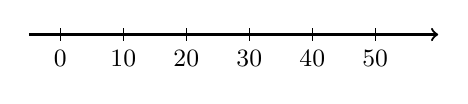
\begin{tikzpicture}[scale=0.08]
  \draw[thick,->] (-5,0) -- (60,0);
  \foreach \x in {0,10,...,55} \draw (\x,1) -- (\x,-1) node[below,font=\small] {$\x$};
\end{tikzpicture}
\end{center}
\end{questionText}
\correctAnswer{$51$ miles from the start}
\explanation{$0 + 35 - 12 + 28 = 51$. The final position is at mile $51$.}
\end{practiceQuestion}
